\documentclass[11pt,a4paper]{article}
\usepackage[T1]{fontenc}
\usepackage[margin=2.3cm]{geometry}
\usepackage{amsmath,amssymb}
\usepackage{graphicx}
\usepackage[dvipsnames]{xcolor}
\usepackage{enumitem}
\usepackage[colorlinks=true,linkcolor=blue,urlcolor=blue]{hyperref}
\setlength{\parskip}{0.6em}
\setlength{\parindent}{0pt}
\begin{document}

\begin{center}{\LARGE\bfseries openflame}\\[0.4em]{\large Measure a flame from a phone video: height, flicker and how far to trust them.}\\[0.2em]\small PAN IIT OSS explainer \textbullet{} higher secondary to advanced undergraduate (levels 4-6)\end{center}

\section*{Why this exists}
A flame on video is a stack of pictures in which a brightness threshold finds the tip, and the tip's height over time is a signal. This explainer shows how a threshold, a Fourier transform and a test on a synthetic video turn such a stack into a height and a flicker frequency with an error bar.

\section*{The end goal}
Measure flame height and flicker frequency from a phone video. The end goal is to measure flame height and flicker frequency from a phone video, and to know how far to trust the numbers. The same ideas drive laboratory combustion diagnostics, the study of pulsating flows and any measurement of an oscillation from a camera.

\section*{How the three sessions build up}
\begin{enumerate}[nosep]
\item \textbf{Session 1: A flame video is a stack of pictures} (Level 1, conceptual interactive model, 60 min).
\item \textbf{Session 2: How fast does it flicker? Sampling and the FFT} (Level 2, mathematical engineering model, 75 min).
\item \textbf{Session 3: Test the whole measurement on a video you know} (Level 3, simulation and validation, 90 min).
\end{enumerate}

\section{Session 1: A flame video is a stack of pictures}

\subsection*{A. Real-world problem}
You film a candle-sized or campfire-sized flame with a phone and ask: how tall is it? The flame never holds still, so a ruler and a stopwatch are no use. But a video is only many still pictures, and a computer can measure the same flame in every one of them. How does a computer decide which pixels are flame, and how does it turn pixels into millimetres? (This repo is general education about image measurement. Do not light fires to experiment unless an adult is present and it is safe.)

\subsection*{B. Concept and theory}
A grey-scale picture is a grid of numbers, one per pixel, from 0 (black) to 1 (white). A video is a stack of such grids, one per frame, so its array has shape (frames, rows, columns). A flame tip is not a sharp edge: the brightness fades over a few pixels. To measure a height we must therefore choose a threshold: a pixel belongs to the flame if its brightness is at least the threshold. Walking up the flame axis from the burner, the measured height is the last pixel that passes. If the brightness on the axis is a smooth fall-off with half-brightness point at height h and softness s, a threshold thr puts the tip at h + s ln((1 - thr)/thr): exactly h at thr = 0.5, higher for a lower threshold, lower for a higher one. A ruler beside the flame gives the scale in millimetres per pixel, which turns pixels into millimetres.

\begin{itemize}[nosep]
\item h: true flame height: the height where the axis brightness is one half (px)
\item z: height above the burner row, counted in pixels (px)
\item s: softness of the tip (pixels over which the brightness fades) (px)
\item thr: brightness threshold, as a fraction of full brightness (no unit)
\item scale: millimetres per pixel (ruler length in mm divided by its length in px) (mm/px)
\item H: measured flame height (px or mm)
\end{itemize}

\begin{equation*}
I(z)=\frac{1}{1+e^{(z-h)/s}}\qquad I(h)=\tfrac12
\end{equation*}

\begin{equation*}
\text{flame pixel}\iff I\ge \mathrm{thr}
\end{equation*}

\begin{equation*}
z_{\mathrm{tip}}=h+s\ln\frac{1-\mathrm{thr}}{\mathrm{thr}}
\end{equation*}

\begin{equation*}
\mathrm{scale}=\frac{L_{\mathrm{ruler}}\ (\mathrm{mm})}{L_{\mathrm{ruler}}\ (\mathrm{px})},\qquad H_{\mathrm{mm}}=H_{\mathrm{px}}\times\mathrm{scale}
\end{equation*}

\begin{center}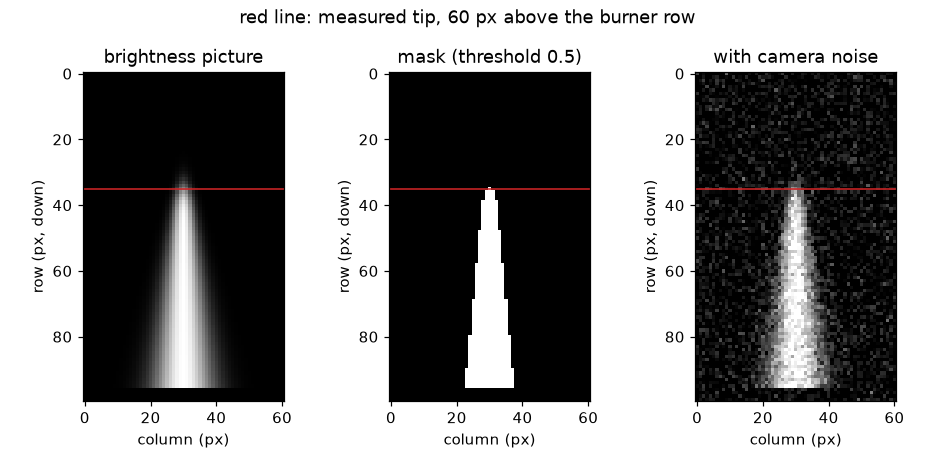
\includegraphics[width=0.85\linewidth]{figures/s01_frame_mask.png}\\\small One synthetic frame, its mask at threshold 0.5 and a noisy frame; the red line is the measured tip.\end{center}

\subsection*{E. Worked example}
A ruler beside the flame is 100 px long in the picture and is 50 mm long. The flame in a frame has its half-brightness tip 60 px above the burner row. What height do you measure at threshold 0.5, in pixels and in millimetres? What would threshold 0.2 have given?
\begin{enumerate}[nosep]
\item Scale = 50 mm / 100 px = 0.5 mm per pixel.
\item At threshold 0.5 the tip is at z = h + s ln(1) = 60 px, so the mask reaches 60 px above the burner row.
\item Height = 60 px x 0.5 mm/px = 30 mm.
\item At threshold 0.2 (s = 2 px) the tip is at 60 + 2 ln 4 = 60 + 2.77 = 62.77 px, and the last whole pixel that passes is 62 px = 31 mm.
\item Sanity check: a candle flame is a few centimetres tall, so 30 mm is plausible; the two thresholds differ by 1 mm, about the size of the tip's own fuzziness.
\end{enumerate}
\textbf{Answer.} At threshold 0.5 the height is 60 px = 30 mm; threshold 0.2 would give 62 px = 31 mm.

\subsection*{F. Questions}
\begin{enumerate}[nosep]
\item \textbf{Conceptual.} Why does a lower threshold give a taller flame? Is there a 'correct' threshold?
\item \textbf{Numerical.} A ruler is 150 px long in the picture and 60 mm long in reality. A flame is 72 px tall at threshold 0.5. How tall is it in mm, and what is the uncertainty if the tip is uncertain by +-1 px?
\item \textbf{Graph and simulation interpretation.} In the threshold figure, what height is measured at thresholds 0.2 and 0.8, and how many millimetres apart are they at 0.5 mm/px?
\item \textbf{Design and optimisation challenge.} Design: for a flame with true height 60 px and softness 2 px, which thresholds measure the height within +-1 px of the truth? Pick one and justify your choice, with noise in mind.
\end{enumerate}

\section{Session 2: How fast does it flicker? Sampling and the FFT}

\subsection*{A. Real-world problem}
A flame does not only have a height, it breathes: it grows and shrinks a few times a second (it is called puffing). A phone camera takes a snapshot every 1/30 of a second. Can 30 snapshots per second measure the breathing, and what is the fastest flicker the camera can see at all? A flame that flickers faster than the camera can follow does not disappear from the video: it shows up at a wrong, slower frequency. This is the same effect that makes a helicopter rotor or a wagon wheel look slow or backwards in a film.

\subsection*{B. Concept and theory}
Model the flame height as a steady mean plus a sinusoidal flicker, h(t) = h0 + A sin(2 pi f t). The camera sees it only at the frame times t = k/fs. We can estimate f in two ways. (1) Count cycles: the mean-removed signal crosses zero upward once per cycle, so f is the number of complete cycles divided by the time they took. (2) The Fourier transform splits the signal into sinusoids; a flicker appears as a peak in the amplitude spectrum, and a Hann window plus zero-padding gives a clean peak and a fine frequency grid. Two limits apply. A recording of T seconds cannot separate frequencies closer than 1/T hertz, so resolution improves with recording length, not with frame rate. And the highest frequency seen correctly is the Nyquist limit fs/2; a faster flicker f is aliased and appears at \textbar{}f - m fs\textbar{}, m being the whole number nearest to f/fs. Two published correlations give what to expect. Heskestad's correlation gives the mean flame height H of a turbulent buoyant diffusion flame (the height reached half of the time) from the heat release rate Q (kW) and the burner diameter D (m): H = 0.235 Q\textasciicircum{}(2/5) - 1.02 D. Pool fires puff at about f = 1.5/sqrt(D) hertz (D in m). Both are fits to experiments on pool fires and gas burners, not laws: use them for turbulent flames from a burner or pool of roughly 0.1 m across and larger, in still air, and expect scatter of tens of percent. They are not valid for small laminar flames such as a candle, for wind-blown or enclosed fires, or for the correlation outputs at very small Q (a negative H means the formula has left its range). This is a simplified educational model, not a fire-safety design tool.

\begin{itemize}[nosep]
\item h(t): flame height as a function of time (m or px)
\item h0, A: mean height and flicker amplitude (same as h)
\item f: flicker (puffing) frequency (Hz)
\item fs: camera frame rate (frames per second (Hz))
\item T: length of the recording (s)
\item N: number of frames, N = fs T (no unit)
\item Q: heat release rate of the fire (kW)
\item D: burner or pool diameter (m)
\item H: mean flame height (Heskestad) (m)
\end{itemize}

\begin{equation*}
h(t)=h_0+A\sin(2\pi f t),\qquad t_k=k/f_s
\end{equation*}

\begin{equation*}
f\approx\frac{n_{\mathrm{cycles}}}{t_{\mathrm{last}}-t_{\mathrm{first}}}
\end{equation*}

\begin{equation*}
X(f)=\sum_{k=0}^{N-1} w_k\,(h_k-\bar h)\,e^{-i2\pi f k/f_s},\qquad \text{amplitude}=\frac{2|X|}{\sum w_k}
\end{equation*}

\begin{equation*}
\Delta f=\frac1T,\qquad f_{\mathrm{Nyq}}=\frac{f_s}{2},\qquad f_{\mathrm{alias}}=\left|f-m f_s\right|,\ m=\mathrm{round}(f/f_s)
\end{equation*}

\begin{equation*}
H=0.235\,Q^{2/5}-1.02\,D\qquad(H\ \mathrm{in\ m},\ Q\ \mathrm{in\ kW},\ D\ \mathrm{in\ m})
\end{equation*}

\begin{equation*}
f\approx\frac{1.5}{\sqrt{D}}\qquad(f\ \mathrm{in\ Hz},\ D\ \mathrm{in\ m})
\end{equation*}

\begin{center}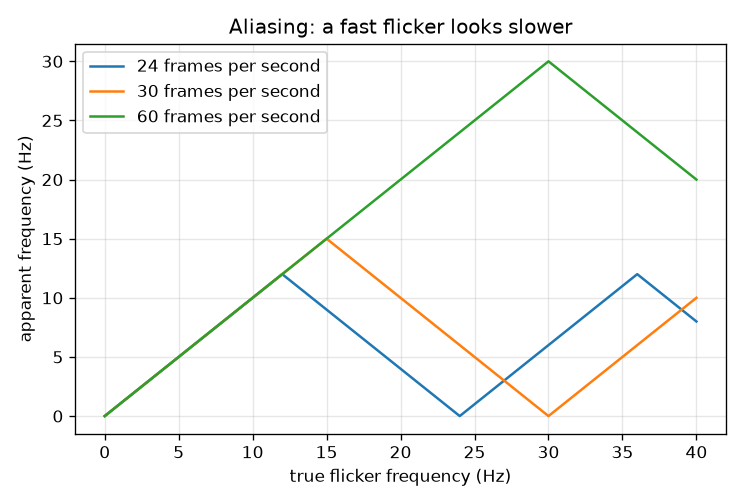
\includegraphics[width=0.85\linewidth]{figures/s02_aliasing_map.png}\\\small Apparent against true flicker frequency for 24, 30 and 60 frames per second: the saw tooth of aliasing.\end{center}

\subsection*{E. Worked example}
A 0.30 m diameter pool fire releases 50 kW. Estimate the mean flame height and the puffing frequency. You film 10 s at 30 frames per second: how many frames, what resolution and what Nyquist limit? Is the flicker seen correctly?
\begin{enumerate}[nosep]
\item Heskestad: 50\textasciicircum{}(2/5) = 4.7818, so 0.235 x 4.7818 = 1.1237 m.
\item Subtract 1.02 x 0.30 = 0.3060 m, so H = 0.8177 m = 0.818 m.
\item Puffing frequency: f = 1.5 / sqrt(0.30) = 1.5 / 0.5477 = 2.74 Hz.
\item Recording: N = 30 x 10 = 300 frames, resolution = 1/10 = 0.1 Hz, Nyquist = 30/2 = 15 Hz.
\item 2.74 Hz is far below 15 Hz, so it is seen correctly and the FFT peak sits within a fraction of 0.1 Hz of it. Sanity check: the flame is about 2.7 burner diameters tall, typical for a pool fire.
\end{enumerate}
\textbf{Answer.} H = 0.818 m and f = 2.74 Hz; the clip has 300 frames, a 0.1 Hz resolution and a 15 Hz Nyquist limit, so the flicker is seen correctly.

\subsection*{F. Questions}
\begin{enumerate}[nosep]
\item \textbf{Conceptual.} A friend films a flame at 24 frames per second and sees a flicker at 9 Hz. Can she conclude the true flicker is 9 Hz?
\item \textbf{Numerical.} A 0.05 m diameter burner puffs at about 1.5/sqrt(D). Calculate that frequency. At what frequency would a camera at 10 frames per second report it, and how does that compare with the Nyquist limit?
\item \textbf{Graph and simulation interpretation.} In the aliasing map, what does a 24 frames per second camera report for a true 20 Hz flicker? Why does the curve return to 0 at 24 Hz?
\item \textbf{Design and optimisation challenge.} Design: you want to measure the puffing frequency of pool fires with diameters from 0.1 m to 1 m to a resolution of 0.05 Hz. Choose a frame rate and a recording length and justify them.
\end{enumerate}

\section{Session 3: Test the whole measurement on a video you know}

\subsection*{A. Real-world problem}
Before you trust a measurement program on a real phone video you must test it on a video whose answer you already know. Is the extracted height right? How accurately is the frequency recovered, and what error bar should you quote? What happens when the frame rate is too low, or the threshold is chosen badly? In this session you build such a test video in code, run the full measurement on it, and break the method on purpose to see where it fails.

\subsection*{B. Concept and theory}
The test video has a known flame height h(t) = h0 + A sin(2 pi f t + phase) (the half-brightness tip) and random camera noise on every pixel. Extraction: average five columns around the flame axis, estimate the flame and background brightness from the whole video, put the threshold a fraction thr between them, walk up from the burner to the first height where three pixels in a row are below it, and interpolate in a straight line to get the tip to a fraction of a pixel. Then fit h0 + a sin + b cos by least squares at trial frequencies near the FFT peak and keep the best: that is the maximum-likelihood frequency for a sinusoid in white noise. Its error is bounded below by the Cramer-Rao bound, which depends on the amplitude A, the residual noise s of the height trace and the number of frames N, and falls as N\textasciicircum{}(-3/2). The threshold shifts the measured height by s\_tip ln((1 - thr)/thr) but does not move the frequency. A frame rate below twice the flicker folds the flicker to an aliased frequency. The error bar assumes white Gaussian noise and a pure sinusoid; a real flame is neither, so a real error bar is larger. It also assumes the fit has found the right peak: when the flicker is weak compared with the noise, some runs lock onto a noise peak and the error bar is meaningless. This is a simplified educational model, not a validated instrument.

\begin{itemize}[nosep]
\item h0, A: mean height and flicker amplitude of the synthetic flame (px)
\item f: flicker frequency (Hz)
\item fs, N: frame rate and number of frames (Hz, no unit)
\item noise: standard deviation of the camera noise per pixel (full brightness is 1) (brightness units)
\item s\_tip: softness of the flame tip (2 px) (px)
\item thr: threshold as a fraction between background and flame brightness (no unit)
\item s: standard deviation of the height-trace residual after fitting (px)
\item sigma\_f: Cramer-Rao standard deviation of the frequency estimate (Hz)
\end{itemize}

\begin{equation*}
h(t_k)=h_0+A\sin(2\pi f t_k+\varphi),\qquad t_k=k/f_s
\end{equation*}

\begin{equation*}
z_{\mathrm{tip}}=h+s_{\mathrm{tip}}\ln\frac{1-\mathrm{thr}}{\mathrm{thr}}
\end{equation*}

\begin{equation*}
\sigma_f=f_s\sqrt{\frac{12}{(2\pi)^2\,\eta\,N(N^2-1)}},\qquad \eta=\frac{A^2}{2s^2}
\end{equation*}

\begin{equation*}
f_{\mathrm{alias}}=\left|f-m f_s\right|,\quad m=\mathrm{round}(f/f_s)
\end{equation*}

\begin{center}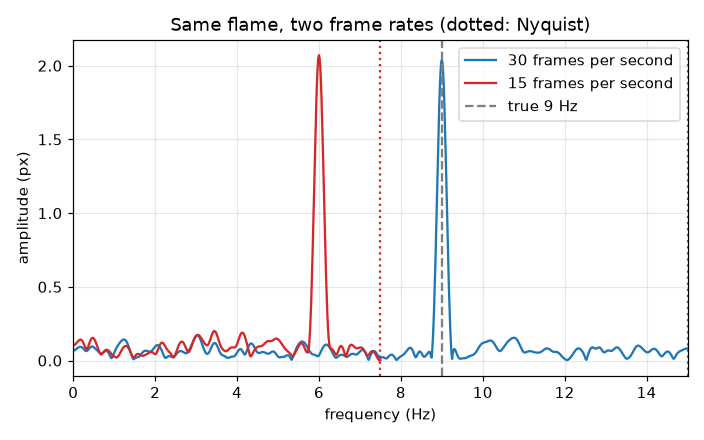
\includegraphics[width=0.85\linewidth]{figures/s03_aliasing_spectra.png}\\\small The same 9 Hz flame filmed at 30 fps (peak at 9 Hz) and 15 fps (peak at the 6 Hz alias).\end{center}

\subsection*{E. Worked example}
A synthetic flame models a 0.30 m pool fire releasing 40 kW, seen by a camera with 13 mm per pixel at 30 frames per second for 8 s, with 2 px flicker amplitude at 2.74 Hz and camera noise 0.15. What mean height (in px) does Heskestad predict? What do the measurements give, and what error bar on the frequency does the formula promise for a residual height noise of 0.44 px?
\begin{enumerate}[nosep]
\item Heskestad: 40\textasciicircum{}(2/5) = 4.3795, so H = 0.235 x 4.3795 - 1.02 x 0.30 = 1.0292 - 0.3060 = 0.7218 m = 722 mm.
\item In pixels: 722 mm / 13 mm per px = 55.5 px. This is the synthetic mean height h0.
\item The video has N = 30 x 8 = 240 frames. The pipeline gives a trace error of 0.41 px (standard deviation) and no bias (+0.05 px), a mean height of 55.56 px = 722 mm, an amplitude of 2.01 px and f = 2.7399 Hz.
\item Error bar by hand: eta = A\textasciicircum{}2 / (2 s\textasciicircum{}2) = 4 / (2 x 0.44\textasciicircum{}2) = 10.33; N(N\textasciicircum{}2 - 1) = 240 x 57599 = 1.382e7; (2 pi)\textasciicircum{}2 = 39.48; so sigma\_f = 30 x sqrt(12 / (39.48 x 10.33 x 1.382e7)) = 30 x 4.61e-5 = 0.0014 Hz.
\item Result: f = 2.7399 +- 0.0013 Hz against the truth 2.74 Hz, within one error bar; the repeated experiments (30 noise seeds) scatter by 0.0013 Hz, matching the formula's 0.0014 Hz.
\end{enumerate}
\textbf{Answer.} The measured mean height is 55.6 px (722 mm), matching Heskestad's 722 mm, and the frequency is 2.740 +- 0.0014 Hz; the error bar is confirmed by 30 repeated experiments.

\subsection*{F. Questions}
\begin{enumerate}[nosep]
\item \textbf{Conceptual.} Why does changing the threshold shift the measured height but hardly change the measured frequency?
\item \textbf{Numerical.} Use the threshold formula for threshold 0.3 and s\_tip = 2 px. How far does the tip move, in px and in mm at 13 mm per px? Is that a large part of the 722 mm flame?
\item \textbf{Graph and simulation interpretation.} In the aliasing spectra figure, the 15 fps spectrum of a 9 Hz flame peaks at 6 Hz. Explain the position of the peak, and say what you would change in the experiment to see 9 Hz.
\item \textbf{Design and optimisation challenge.} Design: you need the flicker frequency to better than 0.01 Hz. At 30 frames per second the flicker amplitude is 1 px and the extraction noise 0.5 px. How long must the recording be? What else would you check?
\end{enumerate}

\section{Real-world mini-project}
\textbf{Measure the flicker of a candle from a phone recording.} A phone recording of a small flame is 12 seconds at 30 frames per second. A ruler held beside the flame gives the scale. Use \texttt{candle\_clip()} from Session 3 as a stand-in (a synthetic candle: 12 s, 30 fps, 0.5 mm per pixel) to build your program first. Then film your own flame only if an adult is present and it is safe to do so: fix the phone on a stand, lock exposure and focus, put a ruler beside the flame, record 12 seconds, extract frames with \texttt{ffmpeg -i clip.mp4 frames/f\%04d.png}, crop them so the flame axis is the middle column, and read them with \texttt{frames\_from\_pngs}. A real candle in still air barely flickers, and a real clip is not a perfect sinusoid, so expect a larger scatter than the synthetic one.

\section{The path ahead}
\begin{enumerate}[nosep]
\item \textbf{Session 4: Glare-corrected height.} An extractor that estimates and subtracts the glare field before thresholding.
\item \textbf{Session 5: Resolve aliasing with two frame rates.} A function that takes two measured apparent frequencies at two frame rates and returns the unique true frequency, or refuses.
\item \textbf{Session 6: The kymograph: convection speed.} A kymograph builder and a stripe-slope estimator.
\item \textbf{Session 7: Detect the onset of flicker.} A sliding-window amplitude estimate with a change-point detector.
\item \textbf{Session 8: A pipeline that refuses to guess.} A measurement wrapper that reads timestamps, calibrates the scale from a ruler frame and refuses a frequency near the Nyquist limit.
\end{enumerate}

\section{Answers and hints}

\subsection*{Session 1}
\begin{enumerate}[nosep]
\item \textbf{Conceptual.} Hint: Where does the brightness at the tip go as you move up? Solution: The brightness fades gradually above the flame, so lowering the threshold lets dimmer, higher pixels count as flame. There is no single correct threshold: the flame has no sharp edge. A threshold is a definition. A good habit is to define the tip as the half-brightness point (threshold 0.5 between background and flame), and to always report the threshold with the height.
\item \textbf{Numerical.} Hint: scale = ruler length in mm divided by ruler length in px. Solution: scale = 60 / 150 = 0.40 mm/px. Height = 72 x 0.40 = 28.8 mm. An uncertainty of +-1 px is +-0.40 mm, so H = 28.8 +- 0.4 mm. Sanity check: the result is a few centimetres, the size of a candle flame.
\item \textbf{Graph and simulation interpretation.} Hint: Read the two heights from the curve and subtract. Solution: At 0.2 the height is 62 px and at 0.8 it is 57 px. The difference is 5 px, which is 5 x 0.5 = 2.5 mm. The curve falls with increasing threshold and crosses the true height (60 px) at threshold 0.5.
\item \textbf{Design and optimisation challenge.} Hint: Solve 59 \textless{}= floor(60 + 2 ln((1 - thr)/thr)) \textless{}= 61 using predicted\_height\_px, or try values. Solution: Thresholds from about 0.27 up to 0.62 give 59 to 61 px (0.27 gives 61, 0.62 gives 59, 0.63 gives 58). Choose about 0.5: it is unbiased by construction, and it sits far from the dark background, so noise specks (which reach a low threshold such as 0.2 first) do not fool the count. Trade-off: a high threshold shortens the flame and loses its dim tip; a low one is easily fooled by noise and glare.
\end{enumerate}

\subsection*{Session 2}
\begin{enumerate}[nosep]
\item \textbf{Conceptual.} Hint: Aliasing: which true frequencies would the camera report as 9 Hz? Solution: Not from this one video. Any true frequency \textbar{}f - m x 24\textbar{} = 9 Hz gives the same picture: 9, 15 (24 - 9), 33 (24 + 9), 39 (48 - 9) and so on. She can only be sure if she knows the flame cannot flicker faster than 12 Hz (the Nyquist limit), or if she films again at a different frame rate and the second apparent frequency is consistent with only one candidate.
\item \textbf{Numerical.} Hint: Nyquist is fs/2; use \textbar{}f - m fs\textbar{} with m = round(f/fs). Solution: f = 1.5 / sqrt(0.05) = 1.5 / 0.2236 = 6.71 Hz. The Nyquist limit at 10 fps is 5 Hz, so 6.71 Hz is aliased: m = round(0.671) = 1 and the apparent frequency is \textbar{}6.71 - 10\textbar{} = 3.29 Hz. (A 0.05 m flame is below the roughly 0.1 m range where the correlation was fitted, so treat 6.71 Hz as a rough guide.)
\item \textbf{Graph and simulation interpretation.} Hint: Find 20 on the horizontal axis of the 24 fps curve. Solution: At 24 fps the curve is \textbar{}20 - 24\textbar{} = 4 Hz at a true 20 Hz. At a true 24 Hz the flicker repeats exactly once per frame, so every frame catches the flame at the same phase: it looks frozen (0 Hz).
\item \textbf{Design and optimisation challenge.} Hint: The flicker frequencies are 1.5/sqrt(D) for the two ends. Resolution is 1/T. Allow a safety margin on the Nyquist limit. Solution: The frequencies are 1.5 / sqrt(0.1) = 4.74 Hz and 1.5 / sqrt(1) = 1.5 Hz. Resolution 0.05 Hz needs T \textgreater{}= 1 / 0.05 = 20 s. Nyquist must exceed 4.74 Hz, so fs \textgreater{} 9.5 Hz; a common 24 or 30 fps camera gives a margin of 2.5 to 3 times and also allows for harmonics. At 24 fps, 20 s is 480 frames. Trade-offs: a longer recording improves resolution only if the flame stays in the same state, and a higher frame rate costs storage and often exposure time without improving resolution.
\end{enumerate}

\subsection*{Session 3}
\begin{enumerate}[nosep]
\item \textbf{Conceptual.} Hint: What does a threshold change in every frame, and what does frequency depend on? Solution: Changing the threshold moves the tip by about the same amount in every frame (s\_tip ln((1 - thr)/thr) for a fixed tip shape), i.e. it adds a nearly constant offset to the whole height trace. Frequency depends on when the height rises and falls, not on its offset, so it is unchanged (the simulation shows 2.739 to 2.741 Hz for thresholds 0.2 to 0.8). The limit: an extreme threshold sits in the noise or inside the flame body and the extraction becomes unreliable.
\item \textbf{Numerical.} Hint: shift = 2 ln((1 - 0.3)/0.3). Solution: shift = 2 ln(0.7/0.3) = 2 x 0.8473 = 1.69 px. In mm: 1.69 x 13 = 22 mm. That is 22/722 = 3 percent of the flame height, small but larger than the 0.4 px trace noise, so the threshold must be reported with the height.
\item \textbf{Graph and simulation interpretation.} Hint: Compare 9 Hz with the Nyquist line of the 15 fps video. Solution: At 15 fps the Nyquist limit is 7.5 Hz and 9 Hz is above it, so it folds to \textbar{}9 - 15\textbar{} = 6 Hz, as the peak shows. To see 9 Hz you must film at more than 18 frames per second (30 fps works), or film at two different frame rates and check which true frequency is consistent with both.
\item \textbf{Design and optimisation challenge.} Hint: Use frequency\_error\_bar(amp, resid\_std, N, fs) for a few values of N and look for sigma\_f below 0.01 Hz. Solution: frequency\_error\_bar gives 0.025 Hz for N = 60 (2 s), 0.0089 Hz for N = 120 (4 s) and 0.0031 Hz for N = 240 (8 s), so at least 4 s meets the target and 8 s gives a margin of three. Also check: the flicker must stay steady over the recording; the amplitude must be well above the noise (at a weak flicker some runs lock onto a noise peak and the formula no longer applies); the frequency must be below the Nyquist limit; and the real error bar is larger than the white-noise one, so a margin is wise.
\end{enumerate}

\section{How to join}
Read \texttt{CONTRIBUTING.md} in the repository, then pick an issue labelled \texttt{good first issue}. Repository: \url{https://github.com/KrunalPanchal1995/openflame}

\end{document}
